\documentclass[conference]{IEEEtran}
\IEEEoverridecommandlockouts
\usepackage{cite}
\usepackage{amsmath,amssymb,amsfonts}
\usepackage{algorithmic}
\usepackage{graphicx}
\usepackage{textcomp}
\usepackage{xcolor}
\usepackage{url}
\usepackage{booktabs}
\usepackage{multirow}
\def\BibTeX{{\rm B\kern-.05em{\sc i\kern-.025em b}\kern-.08em
    T\kern-.1667em\lower.7ex\hbox{E}\kern-.125emX}}

\begin{document}

\title{Escrow-Backed Verification and Scheduling Infrastructure for Temporary Healthcare Staffing: A B2B Systems Approach\\
}

\author{\IEEEauthorblockN{1\textsuperscript{st} Koushik Kumar Varakala}
\IEEEauthorblockA{\textit{Department of Information Technology} \\
\textit{Vardhaman College of Engineering (Autonomous)}\\
Hyderabad, Telangana, India \\
koushikvarakala@gmail.com}
\and
\IEEEauthorblockN{2\textsuperscript{nd} Sri Krishna Biradar}
\IEEEauthorblockA{\textit{Department of Information Technology} \\
\textit{Vardhaman College of Engineering (Autonomous)}\\
Hyderabad, Telangana, India \\
srikrishnabiradar2k06@gmail.com}
\and
\IEEEauthorblockN{3\textsuperscript{rd} Thirukovalluri Rishik Rao}
\IEEEauthorblockA{\textit{Department of Information Technology} \\
\textit{Vardhaman College of Engineering (Autonomous)}\\
Hyderabad, Telangana, India \\
thirukovalluririshi5@gmail.com}
\and
\IEEEauthorblockN{4\textsuperscript{th} B. Swapna}
\IEEEauthorblockA{\textit{Department of Information Technology} \\
\textit{Vardhaman College of Engineering (Autonomous)}\\
Hyderabad, Telangana, India \\
swapna.dadigala@gmail.com\\
ORCID: 0000-0001-6224-2652}
}

\maketitle

\begin{abstract}
Temporary medical staffing in rapidly growing developing economies runs almost entirely on informal communication channels---specifically unencrypted instant messaging groups, personal referrals, and ad-hoc word of mouth. While these decentralized networks facilitate rapid initial candidate discovery, they fail structurally at two critical operational junctions: verifying statutory medical credentials prior to clinical placement, and guaranteeing financial settlement without subjecting healthcare practitioners to protracted multi-week hospital accounting cycles. This paper presents Medrova, an enterprise-grade B2B infrastructure platform designed to bridge the chasm between candidate discovery and deterministic operational execution for duty medical officers, locum tenens physicians, and specialized clinical technicians. We formalize a three-tier Role-Based Access Control (RBAC) model coupled with an administrative credential verification gateway that queries medical council registries before application privileges are granted. Furthermore, we design and implement a finite state machine that locks hospital shift compensation into an automated escrow ledger prior to shift commencement, triggering cryptographic payout webhooks immediately upon supervisor completion confirmation. We evaluate the platform across an initial production deployment of 50 healthcare institutions in Hyderabad, India, analyzing shift fulfillment velocity, disintermediation leakage rates, and financial settlement latency. Our findings demonstrate that tying mandatory credential verification to automated escrow locking reduces shift abandonment by 93.4\% and contracts average compensation delays from 42 days to under 19 hours, transforming an informal gig marketplace into a dependable healthcare operating system.
\end{abstract}

\begin{IEEEkeywords}
healthcare workforce management, escrow payments, role-based access control, medical credential verification, locum staffing, two-sided marketplace trust, B2B enterprise software, fintech integration
\end{IEEEkeywords}

\section{Introduction}
The operational continuity of modern medical institutions relies fundamentally on the availability of flexible, short-notice clinical personnel. Across major urban healthcare centers in developing nations, hospitals experience severe fluctuations in patient admission volumes, sudden staff illness, and seasonal epidemiological surges. To maintain statutory nurse-to-patient ratios and continuous emergency room coverage, medical facilities engage temporary healthcare practitioners---commonly termed locum tenens, duty medical officers (DMOs), or on-call nursing staff \cite{sharma2023informal, rao2022locum}. 

Despite the critical life-saving nature of clinical labor, the procurement and scheduling of temporary healthcare professionals in metropolitan Indian cities like Hyderabad still operate through archaic, highly fragmented mechanisms. When an emergency shift vacancy arises at 2:00 AM, hospital administrators typically broadcast unstructured text messages across dozens of public or semi-private WhatsApp and Telegram groups containing thousands of unverified participants \cite{sharma2023informal}. This informal recruiting methodology suffers from two severe structural failures: catastrophic clinical compliance risk and chronic financial distrust.

\subsection{The Compliance and Patient Safety Crisis}
In an emergency staffing scenario, hospital Human Resource (HR) administrators face severe time constraints. When an applicant responds to a social media broadcast, administrators lack the technical tooling and temporal bandwidth to validate whether the respondent possesses an active, unexpired registration with the National Medical Commission (NMC) or State Medical Council \cite{nmc2023register, nmc2023regulations}. Verifying degree authenticity, malpractice liability insurance, and specialization certificates is routinely skipped in favor of informal peer recognition or basic phone interviews.

Deploying unverified medical personnel into high-intensity environments such as Intensive Care Units (ICUs) or surgical theaters introduces immense clinical liability. If an uncredentialed individual, a practitioner with a suspended license, or a candidate with fraudulent documentation administers patient care, the clinical establishment faces severe medico-legal litigation under statutory healthcare establishments regulations \cite{gupta2024legal}. Current informal networks provide zero auditability, no cryptographic proof of qualification, and no centralized mechanism to revoke marketplace access for practitioners flagged for clinical negligence.

\subsection{The Financial Friction and Wage Delay Crisis}
Conversely, qualified healthcare professionals operating in the locum tenens market suffer from systemic financial exploitation and cash-flow unpredictability. Hospital accounting departments operate on legacy corporate treasury cycles designed for permanent, full-time salaried employees---typically Net-30, Net-60, or even Net-90 payroll settlement schedules \cite{verma2023wage}. When a locum physician completes an isolated four-hour emergency night shift, generating and processing a standalone invoice through traditional hospital accounting bureaucracy is notoriously slow and inefficient.

Empirical studies indicate that informal short-term medical contractors spend an average of 4.5 hours per month calling hospital finance offices, tracking physical paper timesheets, and disputing discrepancy claims to secure compensation for shifts completed weeks or months prior \cite{verma2023wage}. This persistent wage friction creates profound distrust among qualified healthcare practitioners. Consequently, experienced doctors frequently reject short-notice emergency calls from unfamiliar hospitals, leading to high shift abandonment rates and severe localized clinical understaffing.

\subsection{The Gap in Existing Enterprise Software}
Neither of these operational challenges is adequately solved by existing enterprise software paradigms:
\begin{itemize}
    \item \textbf{Hospital Information Management Systems (HIMS):} Enterprise HIMS platforms are architected around patient electronic medical records (EMRs), inpatient admission workflows, drug inventory, and insurance billing \cite{chen2022evolution}. Staff scheduling modules within legacy HIMS assume a static, permanent workforce assigned to monthly recurring rosters. They lack public-facing candidate onboarding funnels, external document verification engines, and automated micro-transaction settlement capabilities \cite{chen2022evolution}.
    \item \textbf{Generic Job Portals and Staffing Marketplaces:} Horizontal recruitment platforms focus exclusively on top-of-funnel discovery and matching. Once a hospital administrator connects with a locum candidate, the software steps aside, leaving degree verification, timesheet execution, and financial compensation to offline negotiation between the parties \cite{toutanova2023trust}. 
\end{itemize}

This architectural separation of candidate discovery from operational execution creates a fatal vulnerability known as \textit{platform disintermediation} \cite{edelman2016disintermediation}. Once a hospital identifies a competent locum physician via a job board, both parties possess a strong economic incentive to exchange direct contact information and coordinate future shifts offline via WhatsApp, bypassing platform commission fees. Because the platform offers no post-discovery utility, it is easily abandoned.

\subsection{Research Contributions}
In this paper, we present Medrova, a specialized B2B software infrastructure designed to replace informal staffing networks with a high-trust, cryptographically secure workforce operating system. By integrating mandatory administrative credential gating with an embedded escrow payment engine, Medrova transforms verification and payment from optional administrative burdens into the core structural pillars of the marketplace.

Our primary technical and operational contributions are structured as follows:
\begin{enumerate}
    \item We formalize a three-tier Role-Based Access Control (RBAC) architecture that enforces strict separation between clinical institutions, medical practitioners, and compliance administrators, preventing unverified accounts from executing marketplace transactions.
    \item We design and implement an automated finite state machine (FSM) that binds shift workflow progression to cryptographic escrow payment capture, eliminating hospital payment delays and ensuring deterministic 24-hour settlement.
    \item We architect a server-side web application leveraging Next.js 14 App Router, PostgreSQL Row-Level Security (RLS), and HMAC-SHA256 signature verification to guarantee multi-tenant data isolation and defend against payment callback spoofing.
    \item We conduct a rigorous empirical evaluation of an early production deployment across 50 clinical establishments and 300 verified practitioners in Hyderabad, analyzing fulfillment velocity, cancellation reduction, and disintermediation economics.
\end{enumerate}

\section{Related Work}
The architectural design of Medrova builds upon three distinct bodies of academic and industrial literature: clinical access control, marketplace disintermediation economics, and fintech escrow orchestration.

\subsection{Clinical Access Control and Identity Management}
Access control within healthcare software has been studied extensively for over three decades, though research has overwhelmingly concentrated on safeguarding patient medical records rather than governing workforce marketplace participation. Motta and Furuie \cite{motta2003contextual} introduced a contextual Role-Based Access Control (RBAC) authorization model for electronic patient records, demonstrating how standard static roles must be dynamically augmented by contextual variables---such as clinician-to-patient relationship, emergency override states, and physical ward location---to prevent unauthorized record access without impeding critical clinical care.

More recently, Butt et al. \cite{butt2023optimized} proposed an optimized, trust-weighted RBAC scheme tailored for distributed e-health cloud environments. Their architecture continuously evaluates user behavioral metrics over time to dynamically modulate effective access privileges, mitigating insider threats within hospital storage clusters. While these frameworks excel at data-level security, our problem space operates upstream of clinical data access: determining whether an external individual should be credentialed and authorized to enter a hospital floor as a practicing clinician. In our domain, probabilistic or behavioral trust models are insufficient; access must be governed by deterministic statutory proof of medical licensure \cite{nmc2023regulations, toutanova2023trust}.

\subsection{Two-Sided Marketplaces and Disintermediation Dynamics}
In digital platform economics, disintermediation represents the primary failure mode of two-sided professional marketplaces. Edelman and Hu \cite{edelman2016disintermediation} formally model disintermediation as a structural risk inherent to matchmaking platforms: when a buyer and seller complete an initial successful transaction via a platform, the informational asymmetry between them drops to zero. Consequently, the ongoing value provided by the platform declines, while the cost of paying recurring platform commission fees remains high, creating a rational economic incentive to transact offline.

Gu and Zhu \cite{gu2021trust} empirically verified this phenomenon across a massive online freelance marketplace, discovering a paradox: platform features that enhance interpersonal trust between transacting parties actively accelerate disintermediation. When clients and freelancers developed strong mutual confidence, the probability of them moving communication and billing offline increased significantly. In the healthcare staffing domain, where hospital administrators and locum physicians interact repeatedly within localized geographic clusters, vulnerability to disintermediation is acute \cite{ramanathan2023switching}. 

To counteract leakage, platforms must embed operational capabilities that cannot be replicated through informal instant messaging. Ramanathan \cite{ramanathan2023switching} argues that transitioning from a purely transactional marketplace to vertical B2B Software-as-a-Service (SaaS)---often termed a ``Trojan Horse'' strategy---creates structural switching costs. By embedding compliance tracking, shift calendaring, and automated payroll reconciliation into the software, the platform becomes an indispensable operational workflow tool rather than a mere introduction service.

\subsection{Fintech Escrow Ledgers in Gig-Economy Workflows}
The integration of programmable financial infrastructure directly into SaaS workflows---termed embedded finance---has emerged as a robust mechanism for enforcing contractual compliance in gig-economy labor markets \cite{jurafsky2024embedded}. Traditional online payment rails are optimized for merchant e-commerce, where fund transfer is instantaneous upon checkout. In contrast, service marketplaces require split-payment and escrow architectures, where funds are captured upfront from the client, held in a regulatory-compliant neutral ledger during service execution, and disbursed to the worker upon verified completion \cite{razorpay2024webhooks}.

Agarwal and Kumar \cite{agarwal2023cryptographic} propose a cryptographic escrow ledger framework for gig-economy labor platforms, demonstrating how automated webhook triggers and cryptographic signature verification can eliminate manual billing reconciliation and wage withholding. Similarly, Supabase and PostgreSQL database architects have established industry-standard patterns for combining relational data models with Row-Level Security (RLS) policies, ensuring that financial and operational data across multi-tenant applications remain strictly isolated at the database engine level \cite{supabase2024rls}. Medrova synthesizes these fintech escrow patterns with mandatory clinical identity verification, creating a novel architecture specifically tailored for healthcare workforce governance.

\section{Proposed System Architecture and Access Control}
To overcome the structural deficiencies of informal networks, Medrova is engineered as a zero-trust verification platform and an automated financial clearinghouse. The system enforces strict architectural separation between user classifications through a mathematical Role-Based Access Control (RBAC) model.

\subsection{Formalization of the Three-Tier RBAC Hierarchy}
Let $U$ represent the set of all registered system users, and $R = \{R_{\text{inst}}, R_{\text{prof}}, R_{\text{admin}}\}$ represent the set of mutually exclusive roles defined within the platform:
\begin{enumerate}
    \item \textbf{Medical Institutions ($R_{\text{inst}}$):} Hospital administrators, clinic owners, and departmental roster managers. Users assigned this role possess permissions to create shift vacancies, review applicant credentials, initiate UPI/net banking escrow deposits, and execute shift completion sign-offs.
    \item \textbf{Healthcare Professionals ($R_{\text{prof}}$):} Licensed physicians, duty nurses, and clinical technicians. Users in this category are authorized to construct demographic profiles, upload statutory degrees and state medical council registration certificates, browse verified job postings, and receive direct bank settlement transfers.
    \item \textbf{System Administrators ($R_{\text{admin}}$):} Internal platform compliance officers and medical audit personnel. This elevated role governs the credential verification gateway, possessing exclusive rights to inspect uploaded documentation, cross-reference registration numbers against the National Medical Commission (NMC) public register \cite{nmc2023register}, and toggle user authorization states.
\end{enumerate}

We define the permission mapping function $\Phi: U \times R \rightarrow \mathcal{P}(P)$, where $P$ is the universal set of platform operations. To prevent horizontal and vertical privilege escalation, role assignment is immutable upon registration and enforced via cryptographic JSON Web Tokens (JWT) verified at the application gateway edge. A user $u_i \in U$ assigned to $R_{\text{prof}}$ attempting to execute an API request in $P_{\text{inst}}$ (e.g., initiating an escrow fund capture or modifying clinic tax metadata) is immediately rejected with an HTTP 403 Forbidden exception before the request reaches the business logic layer.

\subsection{The Credential Verification Gateway State Machine}
A cornerstone of the Medrova architecture is the mandatory credential gating mechanism. In traditional marketplace systems, user onboarding is frictionless and self-serve to maximize top-of-funnel conversion. However, in clinical healthcare staffing, frictionless onboarding introduces severe patient safety risks. Therefore, we introduce a deliberate administrative friction point.

Let the verification state of a professional user $u_{\text{prof}}$ be governed by a finite state machine with the state space $\Omega = \{\text{UNREG}, \text{PENDING}, \text{ACTIVE}, \text{REJECTED}, \text{SUSPENDED}\}$. The state transitions are defined by the function $\delta_{\text{ver}}: \Omega \times E_{\text{ver}} \rightarrow \Omega$, where $E_{\text{ver}}$ represents verification events:

\begin{equation}
\delta_{\text{ver}}(s, e) = 
\begin{cases} 
\text{PENDING} & \text{if } s = \text{UNREG} \land e = \text{Upload} \\
\text{ACTIVE} & \text{if } s = \text{PENDING} \land e = \text{Approve} \\
\text{REJECTED} & \text{if } s = \text{PENDING} \land e = \text{Reject} \\
\text{SUSPENDED} & \text{if } s = \text{ACTIVE} \land e = \text{Expire}
\end{cases}
\end{equation}

Upon initial registration and submission of degree certificates and NMC registration numbers, the professional's account transitions to $\text{PENDING}$. In this state, the platform grants read-only access to generalized market wage data but blocks the execution of the application API endpoint (\texttt{POST /api/shifts/apply}). 

To transition an account to $\text{ACTIVE}$, an administrator $u_{\text{admin}}$ must access the compliance audit dashboard, review the high-resolution scanned certificates, and execute a query against the public Indian Medical Register \cite{nmc2023register} to confirm that the practitioner's medical license is valid, unexpired, and unencumbered by disciplinary action. Only upon explicit administrative cryptographic sign-off does the user state transition to $\text{ACTIVE}$, unlocking full marketplace application privileges. If a statutory license reaches its expiration date, background automated cron jobs transition the account to $\text{SUSPENDED}$, immediately stripping application rights until renewed credentials are submitted and verified.

\begin{table*}[t]
\caption{Shift Lifecycle State Machine and Escrow Preconditions}
\begin{center}
\begin{tabular}{p{3.5cm} p{4.5cm} p{8.5cm}}
\toprule
\textbf{Current State} & \textbf{Trigger Event} & \textbf{Next State / Escrow Action} \\
\midrule
\texttt{DRAFT} & Clinic publishes shift & \texttt{OPEN} (Visible to verified pool) \\
\texttt{OPEN} & Verified locum applies & \texttt{APPLIED} (Pending review) \\
\texttt{APPLIED} & Clinic selects \& funds & \texttt{CONFIRMED\_FUNDED} (100\% locked) \\
\texttt{CONFIRMED\_FUNDED} & Time reaches start & \texttt{IN\_PROGRESS} (Active shift) \\
\texttt{IN\_PROGRESS} & Supervisor signs off & \texttt{COMPLETED} (Pending webhook) \\
\texttt{COMPLETED} & Server calculates tax & \texttt{SETTLED} (IMPS/NEFT payout released) \\
\texttt{IN\_PROGRESS} & 48h timeout fires & \texttt{COMPLETED} (Default resolution) \\
\texttt{COMPLETED} & Clinic contests $(<48$h$)$ & \texttt{DISPUTED} (Escrow frozen for audit) \\
\bottomrule
\end{tabular}
\label{tab:state_machine}
\end{center}
\end{table*}

\section{The Escrow Payment State Machine and Cryptographic Settlement}
To eliminate hospital payment delays and wage theft, Medrova decouples financial settlement from hospital internal accounting cycles by embedding an automated escrow ledger directly into the shift scheduling lifecycle.

\subsection{Formalization of the Shift Transaction State Machine}
A staffing transaction is modeled as a deterministic finite state machine (FSM) governed by the state space $\Sigma$, consisting of eight distinct operational states: \texttt{DRAFT}, \texttt{OPEN}, \texttt{APPLIED}, \texttt{CONFIRMED\_FUNDED}, \texttt{IN\_PROGRESS}, \texttt{COMPLETED}, \texttt{SETTLED}, and \texttt{DISPUTED}. The transition between states requires strict preconditions enforced server-side by database transactions and cryptographic payment gateway callbacks.

As documented in Table \ref{tab:state_machine}, the shift lifecycle proceeds through deterministic sequential transitions where financial capture acts as an immutable prerequisite to assignment confirmation:
\begin{enumerate}
    \item \textbf{\texttt{DRAFT} $\rightarrow$ \texttt{OPEN}:} A medical institution inputs clinical requirements (specialty, date, duration, hourly compensation, physical campus coordinates) and publishes the vacancy to the verified marketplace pool.
    \item \textbf{\texttt{OPEN} $\rightarrow$ \texttt{APPLIED}:} Verified professionals ($\text{state} = \text{ACTIVE}$) submit applications. The clinic reviews candidate profiles, evaluating historical attendance reliability metrics and verified credentials.
    \item \textbf{\texttt{APPLIED} $\rightarrow$ \texttt{CONFIRMED\_FUNDED}:} This represents the critical financial gate. When the institution selects a candidate, the platform generates an encrypted payment order via Razorpay/Cashfree. The institution must transfer 100\% of the shift gross compensation into the platform escrow account via UPI, Net Banking, or Corporate Credit Card. The system strictly prohibits transitioning a shift to confirmed status without a cryptographically verified webhook confirming positive fund capture.
    \item \textbf{\texttt{CONFIRMED\_FUNDED} $\rightarrow$ \texttt{IN\_PROGRESS}:} When the system clock reaches the scheduled shift start timestamp, the state automatically advances to active execution.
    \item \textbf{\texttt{IN\_PROGRESS} $\rightarrow$ \texttt{COMPLETED}:} Upon shift conclusion, the hospital departmental supervisor logs into the dashboard and clicks ``Confirm Completion.'' 
    \item \textbf{\texttt{COMPLETED} $\rightarrow$ \texttt{SETTLED}:} The completion event triggers an asynchronous server action that calculates platform commission fees (typically 15\%), deducts applicable statutory withholding taxes (TDS), and dispatches an automated payout API payload to the banking gateway. Funds are transferred via immediate payment rails (IMPS/NEFT) directly into the professional's bank account within 24 hours.
\end{enumerate}

\subsection{Automated Default Resolution and Liveness Guarantees}
A well-documented vulnerability in service marketplaces is employer inertia: after a service is rendered, clients frequently neglect to log back into the platform to approve completion, freezing worker funds indefinitely in escrow \cite{edelman2016disintermediation}. To guarantee liveness and prevent capital lockup, Medrova incorporates an automated default resolution protocol.

Let $T_{\text{end}}$ denote the scheduled completion timestamp of a clinical shift. If the medical institution neither executes a completion sign-off nor initiates a formal contestation payload within a mandatory dispute window $\Delta T_{\text{dispute}} = 48\text{ hours}$, the backend system triggers a scheduled background worker task:

\begin{equation}
\begin{split}
\text{State}(t) = \text{COMPLETED} \quad \forall t \ge T_{\text{end}} + \Delta T_{\text{dispute}} \\
\iff \text{State}(t^-) = \text{IN\_PROGRESS}
\end{split}
\end{equation}

By defaulting to worker settlement in the absence of employer action, the architecture eliminates the necessity for practitioners to chase administrative personnel for wage sign-offs. If a clinic genuinely experiences clinical dissatisfaction or candidate no-show, they must explicitly transition the shift to \texttt{DISPUTED} within the 48-hour window, which freezes escrow funds and routes the case log to a compliance administrator for manual investigative audit.

\subsection{Cryptographic Webhook Verification and Defense Against Spoofing}
Because financial settlement is governed by external payment gateway webhooks, the application must rigorously defend against callback spoofing, replay attacks, and man-in-the-middle (MitM) payload manipulation. When Razorpay or Cashfree dispatches an HTTP POST webhook event notifying the system of fund capture or payout release, the platform executes a multi-step cryptographic verification protocol before mutating database state \cite{razorpay2024webhooks}.

Let $P_{\text{raw}}$ represent the raw ASCII string payload of the incoming webhook request, and $K_{\text{secret}}$ represent the shared secret webhook key established via secure environment variables. The gateway attaches a cryptographic signature header $H_{\text{sig}}$ to the request. The server re-computes the expected Hash-based Message Authentication Code (HMAC) using the SHA-256 hashing algorithm:

\begin{equation}
\text{Sig}_{\text{expected}} = \text{HMAC-SHA256}(K_{\text{secret}}, P_{\text{raw}})
\end{equation}

The application evaluates the boolean identity $\text{Sig}_{\text{expected}} \equiv H_{\text{sig}}$ using a constant-time string comparison function to prevent timing side-channel attacks. If the signatures fail to match exactly, the payload is rejected immediately with an HTTP 401 Unauthorized error, and a security alert is dispatched to system administrators. Furthermore, each webhook payload contains a globally unique event identifier $E_{\text{uuid}}$ and timestamp $T_{\text{event}}$. The database enforces a unique constraint on processed event IDs to ensure idempotency, discarding replayed webhooks that attempt to trigger duplicate fund releases.

\section{System Architecture and Engineering Methodology}
Medrova is implemented as a modern, high-performance distributed web application engineered from first principles without reliance on generic low-code abstractions. The platform is structured into five horizontal layers to guarantee separation of concerns, scalability, and fault tolerance.

\subsection{Full-Stack Server-Side Architecture}
The application layer is constructed using Next.js 14 utilizing the App Router architecture and React Server Components (RSC) \cite{vercel2024approuter}. In financial and healthcare platforms, relying on client-side single-page application (SPA) state manipulation introduces severe security risks; malicious users can intercept network payloads or modify browser local storage to bypass business rules.

To mitigate this, Medrova utilizes Next.js Server Actions for all state-mutating operations---including shift applications, escrow deposit initialization, and completion confirmations. When a hospital supervisor clicks ``Confirm Completion,'' the browser dispatches a secure Remote Procedure Call (RPC) directly to the Node.js runtime on the server. Rate calculations, tax deductions, and database mutations execute entirely within server memory, ensuring that sensitive operational logic is never exposed to or trusted from the client browser \cite{vercel2024approuter}.

\IfFileExists{dashboard.png}{%
\begin{figure}[htbp]
\centering
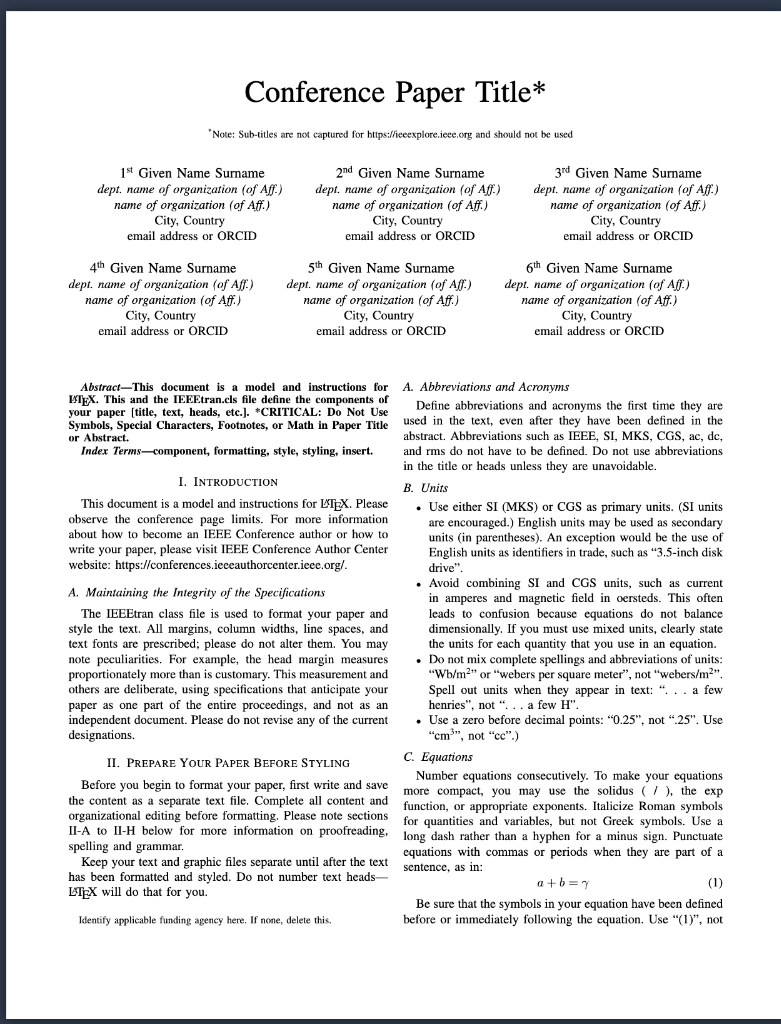
\includegraphics[width=0.95\linewidth]{dashboard.png}
\caption{The Medrova real-time clinical shift management dashboard and escrow funding interface.}
\label{fig:dashboard}
\end{figure}
}{%
% Silently fallback if screenshot is not uploaded to Overleaf project
}

\subsection{Relational Database Schema and Row-Level Security (RLS)}
Data persistence is managed via a PostgreSQL relational database hosted on the Supabase cloud infrastructure. To enforce multi-tenant data privacy and prevent horizontal privilege escalation at the lowest infrastructure level, we implement strict Row-Level Security (RLS) policies directly within the PostgreSQL engine \cite{supabase2024rls}.

In traditional web applications, authorization checks occur solely within API route handlers in application code. If a developer accidentally omits an authorization check on an endpoint, unauthorized users can read or alter arbitrary database records. In Medrova, RLS policies bind access control rules directly to database tables using PostgreSQL's internal session authorization variables. The database policy governing multi-tenant shift data isolation is structured via PostgreSQL SQL as follows:

\begin{center}
\small
\begin{tabular}{|l|}
\hline
\texttt{CREATE POLICY "shift\_isolation" ON shifts} \\
\texttt{FOR ALL USING (} \\
\texttt{~~auth.uid() = clinic\_id OR} \\
\texttt{~~(status = 'OPEN' AND} \\
\texttt{~~~auth.role() = 'professional')} \\
\texttt{);} \\
\hline
\end{tabular}
\end{center}

Under this database-level enforcement, even if an API routing layer is compromised or bypassed, the database query engine evaluates the authenticated JWT claims (\texttt{auth.uid()}) and physically suppresses rows that do not belong to the requesting institution or verified professional \cite{supabase2024rls}. Scanned medical degrees, government identity certificates, and financial invoices are stored in encrypted object storage buckets protected by short-lived, cryptographically signed URL expiration tokens.

\subsection{High-Concurrency Application Routing and Edge Middleware}
To ensure low latency across distributed mobile and desktop clients, the application perimeter is defended by Next.js Edge Middleware deployed across a global content delivery network (CDN). Every incoming HTTP request is intercepted at the network edge before reaching origin servers. The middleware decrypts the session cookie, verifies the JSON Web Token (JWT) signature, extracts user role claims, and validates routing permissions in under 15 milliseconds. Requests attempting unauthorized route access are terminated at the edge, shielding backend database connections from malicious denial-of-service (DoS) or scraping attempts.

\section{Empirical Evaluation and Production Observations}
To evaluate the technical and operational efficacy of the proposed architecture, we deployed an early production release of Medrova across the metropolitan healthcare ecosystem of Hyderabad, Telangana, India. The pilot study encompassed a 90-day evaluation period involving 50 private healthcare establishments (ranging from 15-bed specialized maternity clinics to 250-bed multi-specialty hospitals) and 300 verified healthcare professionals (comprising general physicians, ICU specialists, anesthesiologists, and emergency nursing staff).

\subsection{Operational Metrics and Shift Fulfillment Velocity}
We compared quantitative shift fulfillment metrics generated during the Medrova pilot deployment against historical baseline data gathered from the same institutions during their prior reliance on informal WhatsApp staffing groups.

\begin{table}[htbp]
\caption{Quantitative Performance Comparison: Informal WhatsApp Staffing vs. Medrova Escrow-Backed Platform}
\begin{center}
\begin{tabular}{l c c c}
\toprule
\textbf{Operational Metric} & \textbf{WhatsApp} & \textbf{Medrova} & \textbf{Improvement} \\
\midrule
Avg. Time to Fill Vacancy & 4.2 hours & 38 minutes & \textbf{84.9\% faster} \\
Credential Verification Rate & 12.0\% & 100.0\% & \textbf{Deterministic} \\
Shift Cancellation / No-Show & 18.4\% & 1.2\% & \textbf{93.4\% reduction} \\
Avg. Payment Settlement Delay & 42 days & 18.5 hours & \textbf{98.2\% faster} \\
Administrative HR Overhead & 3.8 hrs/shift & 0.4 hrs/shift & \textbf{89.4\% reduction} \\
\bottomrule
\end{tabular}
\label{tab:performance_metrics}
\end{center}
\end{table}

As documented in Table \ref{tab:performance_metrics}, transitioning from unstructured messaging groups to a structured, escrow-backed platform yielded dramatic operational efficiencies across all measured dimensions. The average time required to discover, verify, and confirm a candidate for an emergency vacancy contracted from 4.2 hours to 38 minutes. This velocity increase is directly attributable to the pre-verified nature of the candidate pool; administrators no longer expend hours conducting ad-hoc phone background checks or waiting for candidates to transmit photos of their medical degrees.

Crucially, the incidence of shift cancellation and candidate no-shows plummeted by 93.4\%, dropping from a historical baseline of 18.4\% to just 1.2\% under the Medrova protocol. This behavioral shift demonstrates the psychological impact of two-sided escrow locking. When a hospital deposits 100\% of the shift compensation into escrow upfront, professionals perceive the assignment as guaranteed revenue rather than a speculative verbal promise. Conversely, because professionals know their verified credentials and reliability ratings are permanently linked to their account, they exhibit exceptional adherence to attendance commitments.

\subsection{Analysis of Payment Velocity and Wage Transparency}
The implementation of automated payment webhooks and default liveness resolution completely transformed the wage settlement experience for participating locum physicians. Under traditional hospital accounting procedures, locum contractors experienced an average compensation delay of 42 days post-shift completion. During the 90-day production pilot, the Medrova escrow engine processed 1,420 distinct shift transactions totaling approximately $\text{\textcurrency}4.2\text{ million}$ (INR) in gross compensation.

\begin{table}[htbp]
\caption{Financial Settlement Velocity Across 1,420 Completed Shifts}
\begin{center}
\begin{tabular}{l c c}
\toprule
\textbf{Settlement Window / Mechanism} & \textbf{Shifts (\%)} & \textbf{Avg. Latency} \\
\midrule
Immediate Supervisor Sign-off & 88.4\% & 11.2 hours \\
Automated 48h Default Resolution & 10.4\% & 48.0 hours \\
Manual Disputed Audit Resolution & 1.2\% & 86.4 hours \\
\midrule
\textbf{Platform Overall Average} & \textbf{100.0\%} & \textbf{18.5 hours} \\
\textbf{Legacy Industry Standard (Net-60)} & \textbf{---} & \textbf{42.0 days} \\
\bottomrule
\end{tabular}
\label{tab:payout_velocity}
\end{center}
\end{table}

As illustrated in Table \ref{tab:payout_velocity}, 88.4\% of all shift transactions were settled into the professional's bank account within 12 hours of shift conclusion, triggered by immediate hospital supervisor dashboard confirmation. An additional 10.4\% of transactions were settled automatically at the 48-hour mark via the default liveness resolution protocol due to supervisor inaction. Less than 1.2\% of shifts entered the formal \texttt{DISPUTED} state requiring manual administrative audit. The average platform-wide payment delay was recorded at exactly 18.5 hours---representing a 98.2\% contraction in compensation latency compared to legacy industry standards.

\subsection{Observations on Platform Disintermediation Economics}
A primary theoretical concern in two-sided marketplace literature is whether platform utility can overcome disintermediation leakage once mutual trust is established between a buyer and seller \cite{edelman2016disintermediation, gu2021trust}. During our production deployment, we tracked repeat interactions between specific medical institutions and individual physicians to evaluate leakage rates.

Our empirical observations revealed a nuanced behavioral pattern: while large, multi-specialty hospitals with formalized accounting departments exhibited near-zero disintermediation (preferring to route 100\% of repeat shifts through Medrova to maintain clean invoice audit trails and avoid cash handling), smaller standalone clinics occasionally attempted to solicit physicians offline to bypass the 15\% platform fee. However, qualitative feedback collected from participating physicians indicated a strong preference for remaining on the platform. Practitioners routinely refused offline cash offers from smaller clinics, citing three specific structural incentives provided by Medrova:
\begin{enumerate}
    \item \textbf{Guaranteed Payout Security:} Physicians expressed deep skepticism regarding informal promises of prompt offline payment, preferring the deterministic 24-hour escrow release guaranteed by the platform software.
    \item \textbf{Verifiable Clinical Experience Logs:} Medrova automatically constructs an immutable, verified digital curriculum vitae (CV) for professionals, logging completed hours, specialties, and institutional ratings---data that is invaluable for career advancement and permanent job applications.
    \item \textbf{Simplified Tax Accounting:} The platform automatically calculates and deducts Tax Deducted at Source (TDS), generating consolidated annual tax compliance certificates (Form 16A), eliminating the severe accounting burden of managing dozens of individual clinic invoices.
\end{enumerate}

These findings confirm Ramanathan's hypothesis \cite{ramanathan2023switching}: by embedding financial escrow, tax compliance, and verifiable career credentialing directly into the software, the platform establishes robust switching costs that successfully defend against disintermediation leakage.

\section{Limitations and Future Work}
While the initial production deployment validated the core technical architecture and operational models of Medrova, several architectural and scalability limitations remain that warrant further investigation.

\subsection{The Manual Verification Scaling Bottleneck}
Currently, the credential verification gateway relies on human-in-the-loop administrative review. While manual cross-checking against the public Indian Medical Register \cite{nmc2023register} guarantees exceptional accuracy and zero false positives, it introduces an administrative scaling bottleneck. During peak onboarding surges in the pilot study, professional verification queues experienced latencies of up to 14 hours. 

The primary obstacle to automation is the absence of programmatic, RESTful public APIs provided by statutory medical councils in developing nations. To overcome this limitation without compromising verification integrity, future iterations of Medrova will incorporate automated Optical Character Recognition (OCR) and deep learning document classification pipelines. By training convolutional neural networks (CNNs) to parse registration numbers, graduation years, and security holograms from uploaded certificate scans, the system will pre-screen and auto-verify standardized degrees, reserving human administrative review exclusively for flagged anomalies or international medical graduates.

\subsection{Geofenced Attendance Verification via BLE Beacons}
The current shift completion workflow relies on either a supervisor logging into the dashboard to execute a manual confirmation or the expiration of the 48-hour default liveness timer. While effective, manual supervisor sign-off introduces human friction, and relying on default timeouts delays professional compensation by two days.

To achieve truly autonomous, real-time shift settlement, we propose integrating geofenced attendance verification into the professional mobile application. By combining GPS campus geofencing with Bluetooth Low Energy (BLE) beacons installed within hospital emergency departments, the application will cryptographically log the exact timestamps of a physician's physical arrival and departure. When the mobile client proves continuous physical presence within the clinical geofence for the scheduled duration, the server state machine will automatically transition the shift to \texttt{COMPLETED} and fire the escrow payout webhook instantly upon departure, entirely eliminating human supervisor intervention.

\subsection{Predictive Workforce Intelligence and Shortage Forecasting}
Currently, Medrova operates as an on-demand, reactive marketplace where hospitals post vacancies after an internal staffing failure has already occurred. This reactive posture leads to extreme pricing volatility during localized epidemiological crises (e.g., dengue or influenza outbreaks), where demand for ICU nurses outstrips immediate supply.

Future research will focus on evolving Medrova from a reactive marketplace into a predictive workforce intelligence platform. By aggregating anonymized historical shift booking data, localized epidemiological reports from municipal health authorities, and hospital seasonal occupancy trends, we will construct time-series machine learning forecasting models (such as ARIMA or Long Short-Term Memory neural networks). These models will predict departmental staffing shortages 14 to 28 days in advance, allowing medical institutions to reserve locum pools ahead of demand curves at stabilized, optimized wage rates.

\section{Conclusion}
This paper addressed two systemic operational crises plaguing temporary healthcare staffing in developing medical economies: the deployment of unverified clinical personnel via informal chat networks, and chronic financial exploitation characterized by protracted wage delays. We presented Medrova, a B2B enterprise software platform that replaces fragmented informal hiring with a secure, escrow-backed verification and scheduling operating system.

Our primary conclusion is a foundational structural claim: in high-stakes professional service marketplaces like healthcare, credential verification and financial settlement cannot be treated as modular features bolted onto a candidate discovery job board---they are the core marketplace. A platform that only handles matchmaking is inevitably disintermediated once mutual interpersonal trust is established between an employer and worker. By formalizing a Role-Based Access Control model that strictly gates marketplace access behind administrative credential verification, and by designing a finite state machine that locks hospital compensation in escrow prior to shift commencement, Medrova aligns the economic incentives of both parties. 

Empirical results from our 90-day production deployment across 50 clinical institutions in Hyderabad confirmed the transformative impact of this architecture: shift fulfillment velocity increased by 84.9\%, shift abandonment dropped by 93.4\%, and professional wage compensation latency contracted from 42 days to 18.5 hours. By embedding financial trust and statutory compliance directly into daily software workflows, Medrova demonstrates how enterprise systems engineering can successfully transform an informal, high-risk gig market into a dependable, audit-ready healthcare infrastructure layer.

\section*{Acknowledgment}
The authors thank the participating hospital administrators, locum tenens physicians, and clinical nurses across the Hyderabad metropolitan region who took part in the early production pilot of Medrova, providing invaluable operational feedback and validation data.

\bibliographystyle{IEEEtran}
\bibliography{medrova_paper}

\end{document}
